\chapter{Adversarial Attacks}
    \section{Contesto teorico}
        Nonostante le reti neurali profonde abbiano raggiunto prestazioni straordinarie in molteplici task visivi, tra cui il riconoscimento facciale, la continua ricerca di tecniche in grado di manipolare l'esito del riconoscimento, le rende potenzialmente vulnerabili ad attacchi di tipo adversarial.
        Gli \textit{adversarial examples} sono immagini appositamente modificate tramite perturbazioni minime e impercettibili per l’occhio umano, in grado di causare un’errata classificazione da parte del modello. Queste perturbazioni sono costruite sfruttando la sensibilità del modello ai gradienti: piccoli cambiamenti nella direzione di maggiore variazione dell’output (calcolati tramite il gradiente della funzione di loss rispetto all’input) possono spostare l’immagine nello spazio delle feature, portando il modello a cambiare la propria predizione anche se, visivamente, l’immagine resta praticamente identica. 
        Questo fenomeno, apparentemente paradossale, è particolarmente preoccupante nell'ambito della cybersecurity, dove il riconoscimento facciale viene utilizzato in sistemi di controllo accessi, autenticazione biometrica, videosorveglianza e verifica dell' identità.
        Esistono due principali categorie di attacco:
            \begin{itemize}
                \item \textbf{Error-generic}: l'obiettivo è far sì che un'immagine venga classificata in una qualsiasi classe diversa da quella corretta.
                
                \item \textbf{Error-specific}: l'obiettivo è far classificare l'immagine in una classe specifica a scelta dell'attaccante.
            \end{itemize}

        \noindent In ambito reale, un attacco error-generic potrebbe portare al rifiuto di accesso per un utente legittimo, mentre un attacco error-specific potrebbe essere usato da un attaccante per impersonare un’altra persona.
        Nel nostro progetto, abbiamo valutato la \textbf{robustezza del modello NN1} attraverso cinque diversi attacchi \textbf{non mirati} (\textit{untargeted}), ovvero attacchi che si limitano a forzare un errore di classificazione, senza specificare la classe obiettivo, e analogamente gli stessi, eccezion fatta per DeepFool, applicati con lo scopo di una misclassificazione verso una specifica classe, quindi \textbf{mirati} (\textit{targeted}).

    \section{Approccio sperimentale}
        Tutti gli attacchi sono stati implementati tramite la libreria \texttt{Adversarial Robustness Toolbox (ART)}. I test sono stati condotti su tutto il test set e per ciascun attacco è stata calcolata la variazione dell’Accuracy top-1 del modello NN1 in funzione del parametro $\epsilon$.
        \textbf{Nota:} Sebbene la traccia del progetto raccomandasse di fermarsi a $\epsilon = 0.05$, abbiamo esteso la sperimentazione includendo i valori:
        
        \[
        \epsilon \in \{0.001,\ 0.005,\ 0.01,\ 0.025,\ 0.05,\ 0.075,\ 0.1\}
        \]
        
        \noindent Questa scelta ha permesso di osservare il comportamento del modello anche oltre i limiti raccomandati, per analizzarne la resistenza in scenari estremi.

    \section{Non-Targeted Adversarial Attacks}
        Gli attacchi non-targeted hanno l'obiettivo di indurre un errore nel classificatore senza forzare la predizione verso una classe specifica, valutandone l'impatto sul classificatore NN1 tramite metriche quantitative e curve di valutazione della sicurezza (\textbf{security evaluation curves}).

        \subsection{Fast Gradient Sign Method (FGSM)}
            Il Fast Gradient Sign Method (FGSM) è un attacco one-shot basato sul gradiente  della funzione di perdita della rete rispetto all'immagine di input. Esso applica una  perturbazione $\epsilon$ proporzionale al segno del gradiente, per allontanarsi dalla classe vera di un $\epsilon$, come mostrato nella seguente formula:
                $$
                x_{\text{adv}} = x + \epsilon \cdot \text{sign}(\nabla_x \mathcal{L}(h(x, w), y))
                $$

            \noindent Nel nostro esperimento, l'attacco è stato eseguito iterando su diversi valori di $\epsilon$:
                $$
                \epsilon \in \{0.001, 0.005, 0.01, 0.025, 0.05, 0.075, 0.1\}
                $$

            \noindent con l'obiettivo di causare una classificazione errata mantenendo una perturbazione impercettibile all'occhio umano, gli adversarial examples sono stati generati a partire dai campioni del test set mediante il FGSM, utilizzando l’implementazione fornita dalla libreria ART. Per ottimizzare l’efficienza computazionale, gli esempi avversari sono stati elaborati in batch di dimensione 64 e successivamente sottoposti al modello NN1 per la fase di inferenza.
            Il processo di valutazione dell’accuratezza segue lo stesso schema già descritto nella sezione precedente, con l’aggiunta di operazioni di normalizzazione e conversione tra tensori e array, necessarie per garantire la compatibilità tra ART e PyTorch.
            Per evitare la rigenerazione degli esempi ad ogni esecuzione, ciascun set avversario è stato salvato su file, con riferimento esplicito al valore di $\epsilon$ utilizzato.
            Infine, il grafico della Security Evaluation Curve mostra l’andamento dell’accuratezza del modello al crescere dell’intensità dell’attacco, evidenziando la relazione inversa tra la robustezza del classificatore e l’entità della perturbazione introdotta.

            \subsubsection*{Risultati sperimentali}
                \noindent L'attacco è stato testato su un range di valori di $\epsilon$. I risultati mostrano un'attesa degradazione delle prestazioni del classificatore NN1 all'aumentare della perturbazione. A partire da $\epsilon$ contenuti il sistema si è dimostrato resiliente agli attacchi, mentre spostandosi ad ordini di grandezza superiori, il modello mostra una vulnerabilità visibile.

                    \begin{itemize}
                        \item $\epsilon = 0.001$: accuratezza 91.28\%, perturbazione media 0.0009
                        
                        \item $\epsilon = 0.010$: accuratezza 44.44\%, perturbazione media 0.0094
                        
                        \item $\epsilon = 0.025$: accuratezza 9.05\%, perturbazione media 0.0235
                        
                        \item $\epsilon = 0.100$: accuratezza 0.46\%, perturbazione media 0.0924
                    \end{itemize}

                \noindent La Security Evaluation Curve mostrata in figura fornisce una rappresentazione visiva chiara dell’impatto degli attacchi FGSM sul modello NN1. La curva mette in evidenza la decrescita in accuratezza del classificatore all’aumentare dell’intensità della perturbazione avversaria.
                In particolare, si osserva una riduzione di oltre il 50\% dell’accuratezza originale per una perturbazione pari a circa 0.01, mentre in corrispondenza del valore massimo consentito ($\epsilon$ = 0.05) mostra un’accuratezza praticamente nulla.

                    \begin{figure}[H]
                        \centering
                        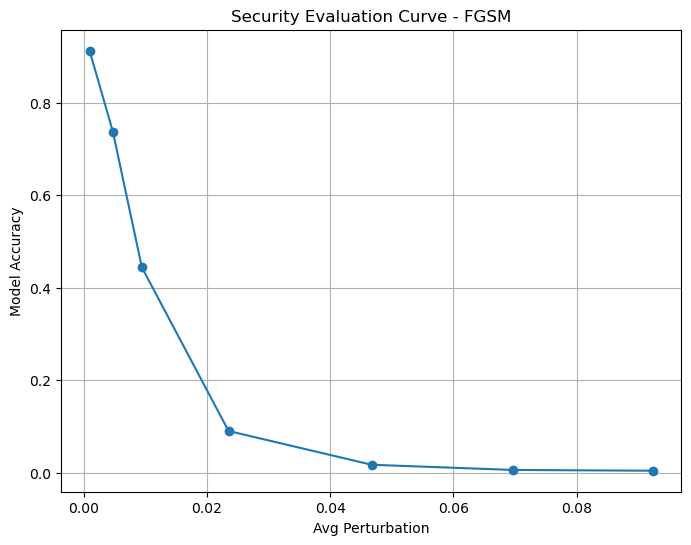
\includegraphics[width=0.65\textwidth]{images/evaluation_curve_fgsm.png}
                        \caption{Security Evaluation Curve per l'attacco FGSM (non-targeted)}
                    \end{figure}

        \subsection{Basic Iterative Method (BIM)}
            Il Basic Iterative Method (BIM) è un'estensione dell'attacco FGSM in cui la perturbazione viene applicata in modo iterativo, con piccoli step e clipping finale per mantenere l'intensità sotto controllo. \\
            La formula iterativa dell’attacco è:
                \[
                x_t' = x_{t-1} + \alpha \cdot \text{sign} \left( \nabla_x \mathcal{L}(h(x_{t-1}, w), y) \right)
                \]

            \noindent dove $\alpha$ è la quantità di rumore aggiunta ad ogni iterazione e $\boldsymbol{t}$  rappresenta il numero di iterazioni. L'idea di aggiungere piccole quantità di rumore in diversi step multipli aumenta le probabilità di misclassificare un'immagine rispetto all'attacco originale.

            \subsubsection*{Risultati sperimentali}
                \noindent Per l'attacco Basic Iterative Method (BIM) sono stati eseguiti esperimenti variando sia il parametro $\epsilon$ sia il numero massimo di iterazioni $t \in \{5, 10, 20\}$. I risultati, in linea con quanto introdotto, evidenziano un chiaro incremento dell'efficacia dell'attacco all'aumentare di entrambi i parametri.
                
                \begin{itemize}
                    \item Per $\epsilon = 0.001$ l’accuratezza rimane invariata intorno al 91.3\%, indipendentemente dal numero di iterazioni.
                    
                    \item Per $\epsilon = 0.01$, l’accuratezza cala drasticamente fino al 20.60\% con $t=20$.
                    
                    \item Per $\epsilon \geq 0.025$, l’accuratezza scende sotto l’1\% già a 5 iterazioni, fino ad azzerarsi con $t \geq 10$.
                \end{itemize}
                
                \noindent L’aumento del numero di iterazioni risulta particolarmente efficace nel regime di $\epsilon$ intermedio (es. 0.01–0.05), mentre a valori molto elevati l’accuratezza crolla anche con pochi passi. La curva mostra come l’attacco riesca a compromettere il modello con perturbazioni limitate ma iterative.

                \begin{figure}[H]
                    \centering
                    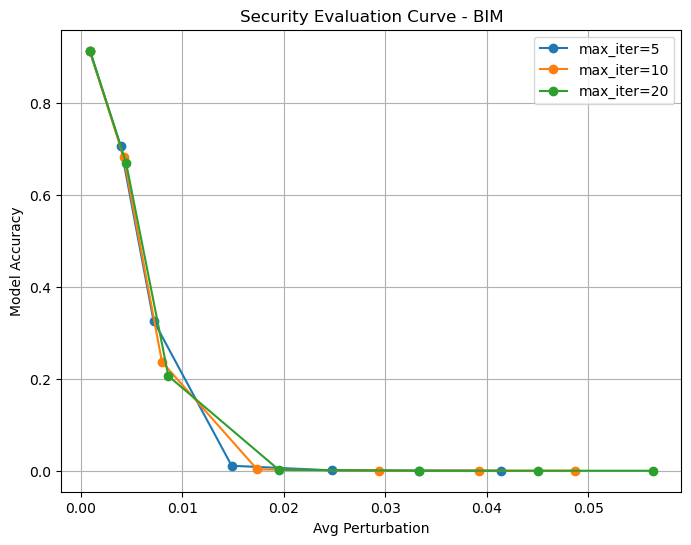
\includegraphics[width=0.75\textwidth]{images/evaluation_curve_bim.png}
                    \caption{Security Evaluation Curve per l'attacco BIM (non-targeted)}
                \end{figure}

                \noindent Analizzando la curva, si osserva che, a parità di accuratezza del modello, un numero maggiore di iterazioni consente di ingannare il classificatore con perturbazioni di intensità inferiore. In particolare, le curve corrispondenti a 10 e 20 iterazioni raggiungono un’accuratezza prossima allo 0\% più rapidamente rispetto a quella relativa a 5 iterazioni, evidenziando una maggiore efficacia dell’attacco al crescere del numero di passi di ottimizzazione.

        \subsection{Projected Gradient Descent (PGD)}
            Il Projected Gradient Descent (PGD) rappresenta una generalizzazione iterativa dell’attacco FGSM. Alla base di PGD c’è l’idea di eseguire piccoli passi iterativi seguendo il gradiente della funzione di perdita rispetto all'input, aggiornando progressivamente l'immagine avversaria. Dopo ogni passo, l’immagine perturbata viene proiettata nuovamente all’interno della sfera di raggio $\epsilon$ centrata sull’immagine originale ($\epsilon$ ball).
            La formula iterativa è simile a quella di BIM, ma include la funzione di proiezione $\pi$ a ogni passo:
            
            \[
            x_t' = \Pi_\epsilon \left( x_{t-1} + \alpha \cdot \text{sign} \left( \nabla_x \mathcal{L}(h(x_{t-1}, w), y) \right) \right)
            \]
            
            \noindent dove $\Pi$ è la funzione di proiezione nella sfera L$_\infty$, $\alpha$ è il passo, e $\mathcal{L}$ la loss.

            \subsubsection*{Risultati sperimentali}
                \noindent L'attacco Projected Gradient Descent (PGD), noto per essere una versione iterativa più robusta del FGSM e di BIM, è stato testato con due valori di iterazioni massime $t \in \{10, 20\}$ e diversi valori di $\epsilon$.
                
                \begin{itemize}
                    \item Per valori molto bassi di $\epsilon$ (0.001), il modello mantiene un’alta accuratezza (91.3\%), anche dopo 20 iterazioni.
                    \item A partire da $\epsilon = 0.01$, l’accuratezza crolla drasticamente, si scende al 25.5\% con $t=10$ e al 20.9\% con $t=20$.
                    \item Per $\epsilon \geq 0.025$, il modello viene completamente compromesso: l’accuratezza si avvicina allo 0\%, anche con perturbazioni medie contenute.
                \end{itemize}
                
                \noindent I risultati dimostrano l’efficacia dell’attacco PGD, in grado di abbattere rapidamente l’accuratezza del classificatore anche con perturbazioni visivamente impercettibili. L’aumento di iterazioni da 10 a 20 migliora leggermente l’efficacia dell’attacco nei range intermedi di $\epsilon$.

                \begin{figure}[H]
                    \centering
                    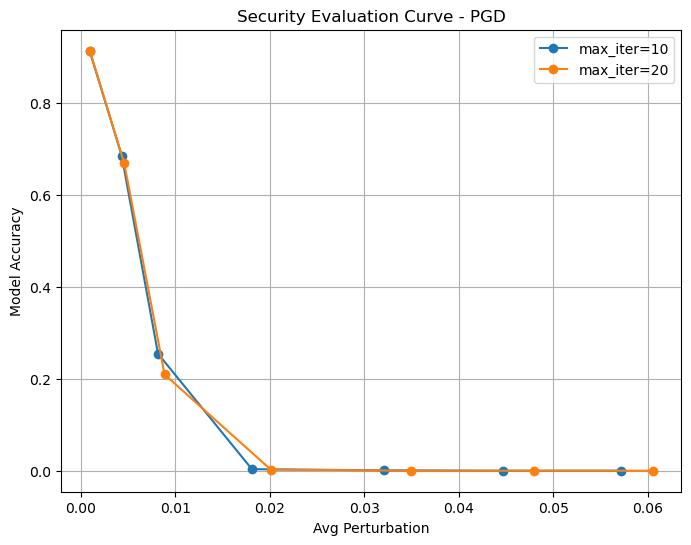
\includegraphics[width=0.75\textwidth]{images/evaluation_curve_pgd.png}
                    \caption{Security Evaluation Curve per l'attacco PGD (non-targeted)}
                \end{figure}

        \subsection{DeepFool}
            L’attacco \textbf{DeepFool} è una tecnica iterativa per la generazione di perturbazioni minime che portino un classificatore lineare, o non, a misclassificare l'output. A differenza degli attacchi gradient-based più aggressivi, come PGD, DeepFool mira specificamente a trovare la perturbazione minima necessaria a spingere l'immagine oltre il confine decisionale del classificatore, rappresentato da un iperpiano, garantendo quindi un attacco più ``preciso'' in termini di ottimizzazione dell'energia della perturbazione. \\
            La formula alla base dell’attacco (nella versione binaria) si ispira a:
                \[
                r^* = - \frac{f(x)}{\| \nabla f(x) \|^2} \cdot \nabla f(x)
                \]
            
            \subsubsection*{Risultati sperimentali}
                \noindent Nel nostro esperimento, abbiamo selezionato \textbf{50 immagini casuali} dal test set, impostando come parametri principali un \textit{overshoot} $\epsilon = 0.02$ e massimo \textit{numero di iterazioni} pari a 5, con i primi 10 gradienti dominanti (classi più probabili) considerati.
                L’accuratezza residua del modello dopo l’attacco è risultata pari a \textbf{84.00\%}, con una \textbf{fooling rate} complessiva del \textbf{16.00\%}. Il valore medio di perturbazione $L\infty$ applicato è stato molto contenuto: \textbf{0.00163}, a conferma della natura parsimoniosa dell’attacco.
                
                \begin{figure}[H]
                    \centering
                    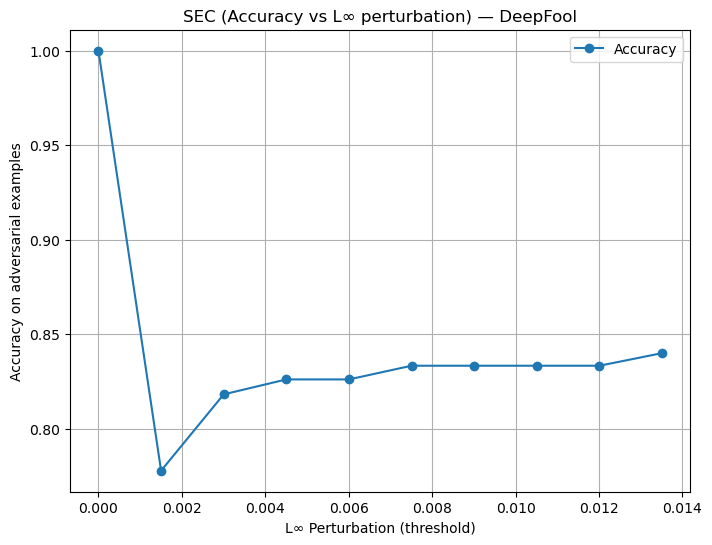
\includegraphics[width=0.6\linewidth]{images/evaluation_curve_deepfool.png}
                    \caption{Security Evaluation Curve (SEC) --- Accuratezza vs. soglia $L\infty$ (DeepFool)}
                \end{figure}
                
                \noindent Nel primo grafico è riportata la \textbf{Security Evaluation Curve (SEC)}, che mostra l’andamento dell’accuratezza del classificatore al variare del valore soglia massimo di perturbazione $L\infty$. Si osserva una prima brusca caduta dell’accuratezza anche per soglie molto piccole, seguita da una stabilizzazione intorno all’83–84\%: questo suggerisce che una porzione delle immagini avversarie riesce ad alterare la previsione già con minime modifiche.
                
                \begin{figure}[H]
                    \centering
                    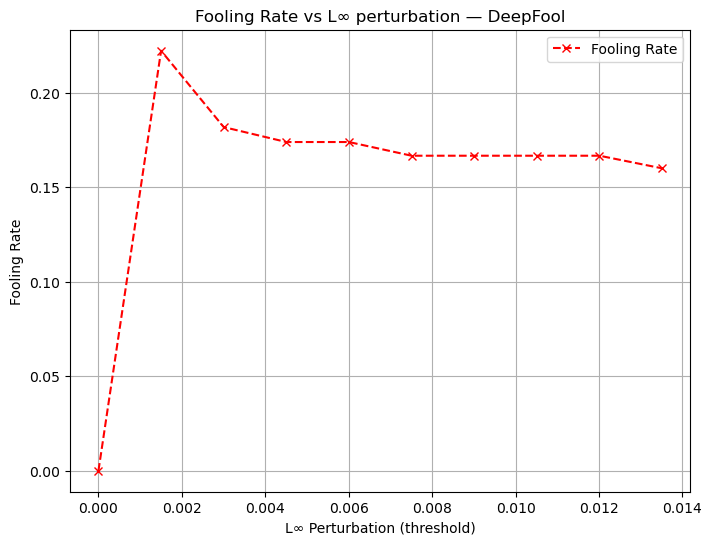
\includegraphics[width=0.6\linewidth]{images/fooling_rate_deepfool.png}
                    \caption{Tasso di inganno (Fooling Rate) vs. soglia $L\infty$ (DeepFool)}
                \end{figure}
                
                \noindent Il secondo grafico mostra la \textbf{fooling rate}, ovvero la percentuale di immagini la cui predizione è stata alterata, rispetto alla soglia massima di perturbazione. Si nota un picco iniziale (oltre il 20\%) per soglie minime, seguito da una graduale decrescita. Questo comportamento è coerente con quanto evidenziato in letteratura, dove viene mostrato come le perturbazioni ottimali di DeepFool tendano a concentrarsi su un sottile margine decisorio, risultando estremamente efficaci anche a bassissime magnitudini. Tuttavia, al crescere della soglia, il numero di immagini ``foolabili'' non aumenta proporzionalmente: ciò indica una certa robustezza intrinseca per una porzione del dataset, o l’inadeguatezza del metodo DeepFool su immagini più complesse (in quanto è un attacco non-targeted e localmente lineare).
                Questo andamento è dunque assolutamente plausibile e rafforza il ruolo di DeepFool come attacco utile per valutare con maggior precisione la vulnerabilità del modello, senza ricorrere a grandi perturbazioni.
            
        \subsection{Carlini-Wagner (CW) $L\infty$}
            \noindent L’attacco Carlini-Wagner (CW) è tra i più noti ed efficaci attacchi basati sul gradiente. Si fonda sulla formulazione di un problema di ottimizzazione vincolata, in cui l’obiettivo è minimizzare l’intensità della perturbazione necessaria a causare una classificazione errata.
            Rispetto ad altri metodi, come DeepFool, l’attacco CW risulta computazionalmente più oneroso, in quanto ad ogni iterazione l’algoritmo esplora diverse regioni di decisione proiettando la perturbazione in ciascuna di esse, confrontandone la distanza dal campione originale per selezionare quella che minimizza la norma del rumore aggiunto.
            Nel caso della norma $L\infty$, il problema si può riassumere come:
            \[
            \min \| \delta \|_\infty \quad \text{such that} \quad f(x + \delta) \ne y
            \]
            
            \noindent In questa sezione valutiamo l'efficacia dell'attacco non-targeted, variando l'apprendimento ($\text{learning\_rate} \in \{0.01, 0.1\}$), la costante iniziale ($\text{init\_const} \in \{0.01, 0.1\}$) e il numero massimo di iterazioni ($\text{max\_iter} \in \{1, 10, 20\}$). I risultati si riferiscono ad un sottoinsieme casuale di 20 immagini selezionate dal test set.
            
            \begin{figure}[H]
                \centering
                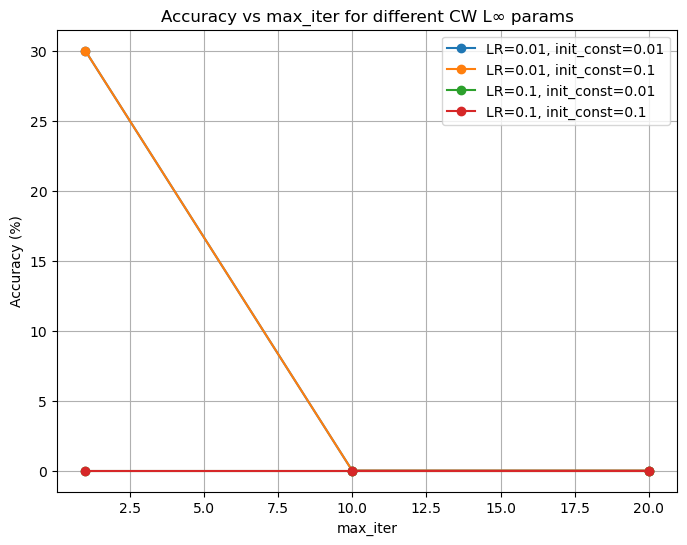
\includegraphics[width=0.65\textwidth]{images/cw_non_targeted_accuracy.png}
                \caption{Accuracy vs \texttt{max\_iter} per diversi parametri dell'attacco CW $L\infty$ (non-targeted).}
                \label{fig:cw-nt-accuracy}
            \end{figure}
            
            \noindent Come visibile in Figura~\ref{fig:cw-nt-accuracy}, l'attacco si dimostra estremamente efficace. Per $\text{learning\_rate} = 0.1$ l’accuratezza del modello scende immediatamente a $0\%$ indipendentemente da $\text{max\_iter}$ e $\text{init\_const}$, mentre con $\text{learning\_rate} = 0.01$ e $\text{max\_iter} = 1$ l’attacco è meno potente, riuscendo a mantenere un’accuratezza residua del $30\%$. Già a $\text{max\_iter} = 10$ l’attacco diventa efficace anche in questo scenario, abbattendo completamente le prestazioni del classificatore.
            
            \begin{figure}[H]
                \centering
                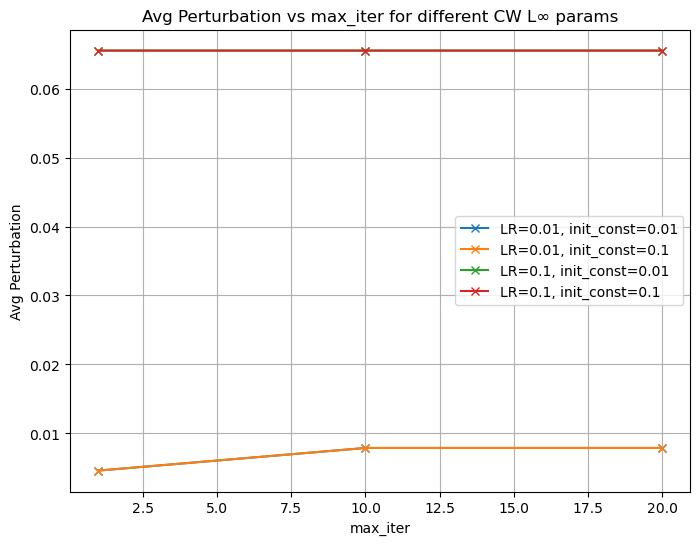
\includegraphics[width=0.65\textwidth]{images/cw_non_targeted_perturbation.png}
                \caption{Avg perturbation vs \texttt{max\_iter} per diversi parametri dell'attacco CW $L\infty$ (non-targeted).}
                \label{fig:cw-nt-perturbation}
            \end{figure}
            
            \noindent La figura~\ref{fig:cw-nt-perturbation} mostra come le perturbazioni siano controllate e in generale molto limitate, soprattutto per $\text{learning\_rate} = 0.01$, dove si rimane sotto lo 0.01 anche a 20 iterazioni. Al contrario, l’uso di un tasso di apprendimento più elevato porta a perturbazioni stabili ma più marcate ($\sim 0.065$), comunque sufficienti per ingannare completamente il modello.
            
            \begin{figure}[H]
                \centering
                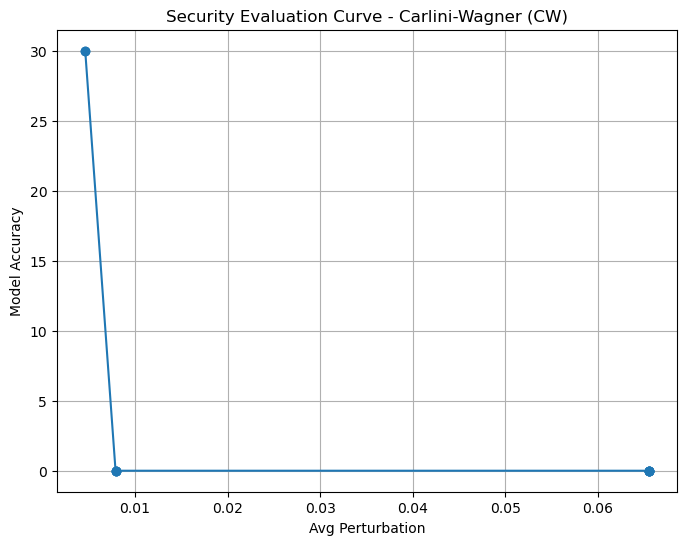
\includegraphics[width=0.65\textwidth]{images/cw_unt_ec.png}
                \caption{Security Evaluation Curve per CW $L\infty$ (non-targeted): accuratezza vs perturbazione media.}
                \label{fig:cw-nt-sec}
            \end{figure}
            
            \noindent La \textbf{Security Evaluation Curve} (Figura~\ref{fig:cw-nt-sec}) evidenzia la forte correlazione inversa tra perturbazione e accuratezza. L’attacco si conferma altamente efficace anche con perturbazioni estremamente contenute: l’unico punto con accuracy significativamente diversa da zero ($30\%$) corrisponde a $\epsilon \approx 0.0046$. Per perturbazioni superiori, l’attacco riesce sistematicamente a compromettere la classificazione.

        \subsection{Carlini-Wagner (CW) $L2$}
            In questo esperimento abbiamo applicato l'attacco Carlini-Wagner nella variante $L2$ e in modalità non-targeted direttamente alla rete NN1. Sono state esplorate diverse configurazioni dei parametri: \texttt{learning\_rate} $\in \{0.01, 0.1\}$, \texttt{initial\_const} $\in \{0.01, 0.1\}$ e \texttt{max\_iter} $\in \{1, 10, 20\}$. I risultati ottenuti sono rappresentati nei grafici in Figura~\ref{fig:cw_untarg_l2_acc}, \ref{fig:cw_untarg_l2_pert} e \ref{fig:cw_untarg_l2_sec}.
            
            \begin{figure}[H]
                \centering
                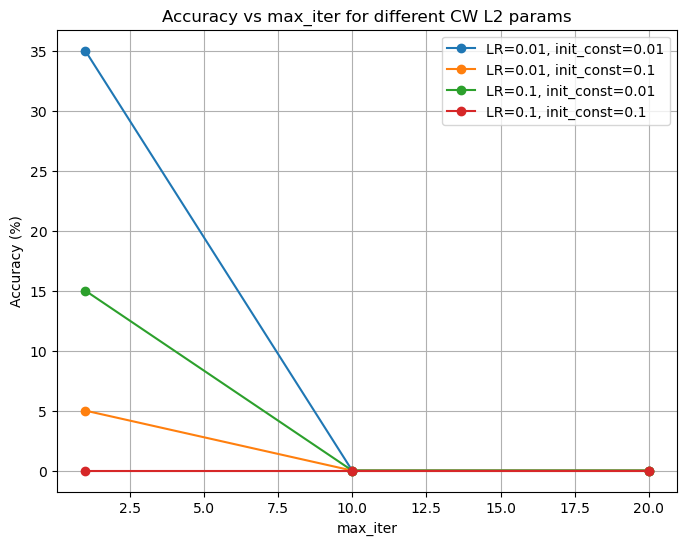
\includegraphics[width=0.6\textwidth]{images/accvsmaxl2.png}
                \caption{Accuracy vs max\_iter per Carlini \& Wagner $L^2$ (Non-targeted, NN1)}
                \label{fig:cw_untarg_l2_acc}
            \end{figure}
            
            \begin{figure}[H]
                \centering
                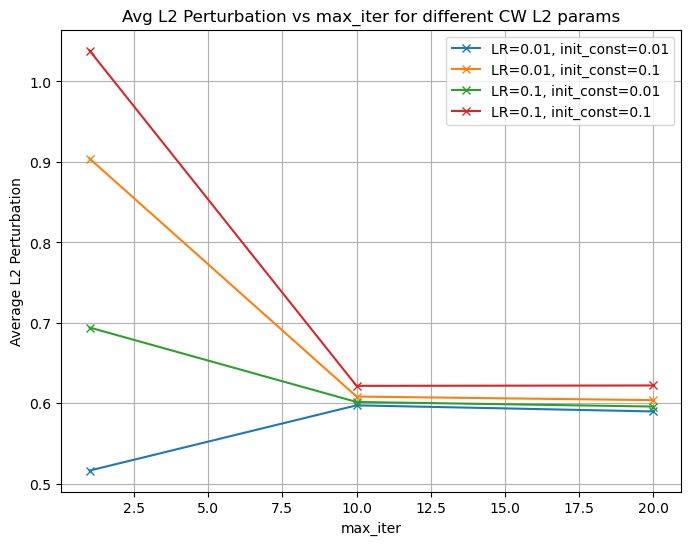
\includegraphics[width=0.6\textwidth]{images/avgpub_vs_maxiter_l2.png}
                \caption{Avg $L^2$ Perturbation vs max\_iter per Carlini \& Wagner $L^2$ (Non-targeted, NN1)}
                \label{fig:cw_untarg_l2_pert}
            \end{figure}
            
            \begin{figure}[H]
                \centering
                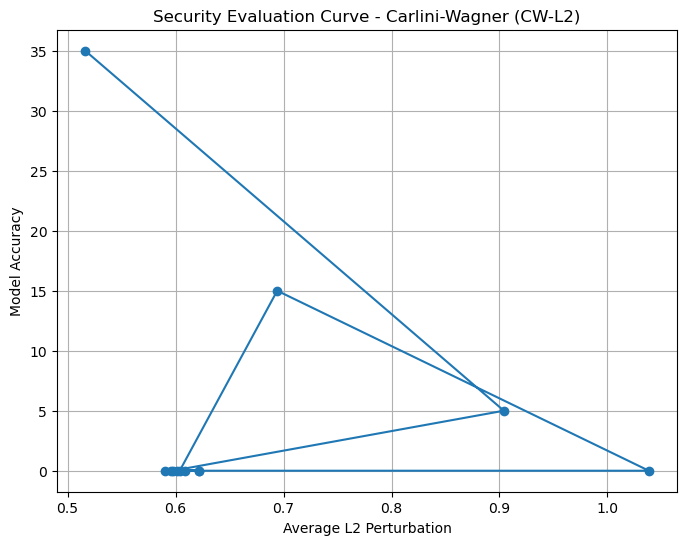
\includegraphics[width=0.6\textwidth]{images/sec_unt_cw_l2.png}
                \caption{Security Evaluation Curve per Carlini \& Wagner $L^2$ (Non-targeted, NN1)}
                \label{fig:cw_untarg_l2_sec}
            \end{figure}
            
            \subsection{Risultati sperimentali}
                L'attacco Carlini-Wagner $L2$ in modalità non-targeted si è dimostrato altamente efficace nel compromettere le predizioni della rete NN1. Per configurazioni con \texttt{max\_iter} elevate, l’accuratezza residua del modello si riduce rapidamente fino allo $0\%$, evidenziando che la rete è completamente ingannata dai campioni avversari generati.
                Nelle configurazioni con \texttt{max\_iter=1}, l’attacco non raggiunge lo stesso livello di successo, ma riesce comunque ad abbattere l'accuratezza fino al $5\%$–$35\%$, in funzione del valore di \texttt{init\_const} e \texttt{learning\_rate}. Al crescere delle iterazioni, l’attacco converge verso perturbazioni più “efficaci” e meno intense, con valori medi di norma $L2$ compresi tra $0.59$ e $0.62$.
                La \textit{security evaluation curve} evidenzia una forte correlazione inversa tra la norma della perturbazione e l’accuratezza del classificatore: perturbazioni anche relativamente modeste sono sufficienti a compromettere il riconoscimento. Questo conferma che CW-$L2$ è uno degli attacchi più performanti contro la rete NN1 in modalità non-targeted, anche senza trasferimento.

    \clearpage

    \section{Targeted Adversarial Attacks}
        Gli attacchi avversari \textbf{targeted} hanno l’obiettivo non solo di causare un errore di classificazione, ma di forzare il classificatore a predire deliberatamente una classe specifica, a scelta dall’attaccante. A differenza degli attacchi error-generic (non-targeted), in cui l’obiettivo è semplicemente a causare una misclassification, gli attacchi targeted mirano a far apparire un esempio come appartenente a una identità arbitraria.
        Nei contesti biometrici, come il face recognition, questi attacchi sono particolarmente pericolosi: un attaccante può modificare la propria immagine in modo tale da essere riconosciuto come un’altra persona autorizzata al sistema. Di conseguenza, gli attacchi targeted pongono una minaccia diretta all’integrità dei sistemi di autenticazione.
        In questa sezione vengono analizzati i principali attacchi targeted testati nella nostra sperimentazione: FGSM, BIM, PGD e CW, adattati nella modalità targeted.

        \subsection{Fast Gradient Sign Method (Targeted)}
            Il \textit{Fast Gradient Sign Method} (FGSM), nella sua variante targeted, genera una perturbazione mirata con l’obiettivo di forzare il classificatore a predire una classe specifica scelta dall’attaccante. A differenza della modalità non-targeted, dove si massimizza la loss rispetto all’etichetta reale, minando quindi la \textit{confidence} del classificatore verso la classe true, in quella targeted si minimizza la loss rispetto all’etichetta obiettivo $y_{\text{target}}$, massimizzando la confidence del classificatore verso la classe target:
            \[
            x_{\text{adv}} = x - \epsilon \cdot \text{sign}\left( \nabla_x \mathcal{L}(h(x, w), y_{\text{target}}) \right)
            \]
            
            \noindent dove $\epsilon$ rappresenta l’intensità della perturbazione e la direzione del gradiente è invertita per avvicinarsi alla classe target.
            Questo tipo di attacco è generalmente più difficile da realizzare rispetto a quello non mirato e la curva di sicurezza ottenuta lo conferma.
            
            \begin{figure}[H]
                \centering
                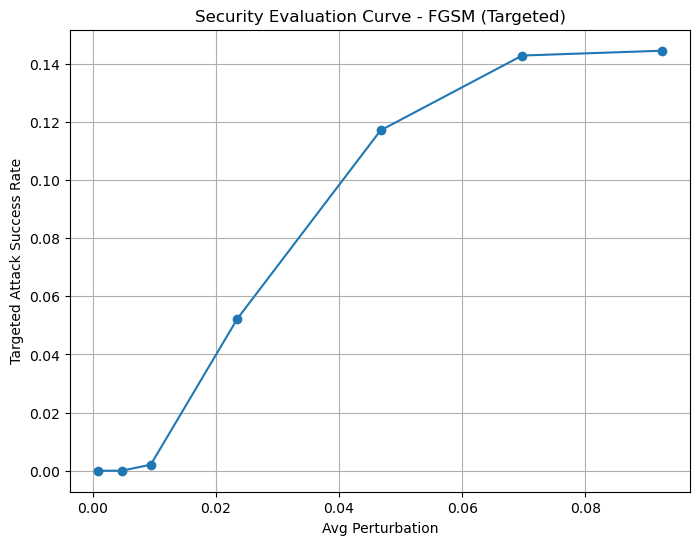
\includegraphics[width=0.65\textwidth]{images/evaluation_curve_fgsm_targeted.png}
                \caption{Security Evaluation Curve per FGSM Targeted. L'asse delle ascisse rappresenta la perturbazione media, mentre l'asse delle ordinate mostra la targeted success rate.}
                \label{fig:fgsm_targeted_curve}
            \end{figure}
            
            \noindent Come si osserva dalla Figura~\ref{fig:fgsm_targeted_curve}, l'efficacia dell'attacco cresce al crescere della perturbazione introdotta, ma in maniera piuttosto contenuta. L'attacco ottiene un successo massimo del 14.45\% per \(\epsilon = 0.1\), confermando che l’FGSM risulta inefficace per attacchi mirati a bassa perturbazione.
            
            \begin{table}[H]
                \centering
                \label{tab:fgsm_targeted}
                \begin{tabular}{c|c|c|c}
                    \toprule
                    \textbf{Epsilon} & \textbf{Perturbazione media} & \(\mathbf{L_\infty}\) & \textbf{Targeted Success Rate} \\
                    \midrule
                    0.001 & 0.0009 & 0.0010 & 0.00\% \\
                    0.005 & 0.0047 & 0.0050 & 0.00\% \\
                    0.010 & 0.0094 & 0.0100 & 0.21\% \\
                    0.025 & 0.0235 & 0.0250 & 5.23\% \\
                    0.050 & 0.0467 & 0.0500 & 11.71\% \\
                    0.075 & 0.0697 & 0.0750 & 14.29\% \\
                    0.100 & 0.0924 & 0.1000 & 14.45\% \\
                    \bottomrule
                \end{tabular}
                \caption{Risultati ottenuti con FGSM targeted.}
            \end{table}

        \subsection{Basic Iterative Method (Targeted)}
            Il \textit{Basic Iterative Method} (BIM) estende FGSM applicando la perturbazione in più passi di piccola entità. Nella modalità targeted, l’attacco forza l'immagine verso una classe obiettivo $y_{\text{target}}$ minimizzando la loss rispetto a tale classe. La formula ricorsiva del metodo è:
            
            \[
            x_t = x_{t-1} - \alpha \cdot \text{sign}\left( \nabla_x \mathcal{L}(h(x_{t-1}, w), y_{\text{target}}) \right)
            \]
            
            \noindent dove $\alpha = \epsilon / T$ rappresenta lo step size e $T$ è il numero totale di step.
            L'attacco  è stato valutato su un ampio spettro di valori del parametro \(\epsilon\), variando anche il numero massimo di iterazioni tra \texttt{5}, \texttt{10} e \texttt{20}. 
            
            \begin{figure}[H]
                \centering
                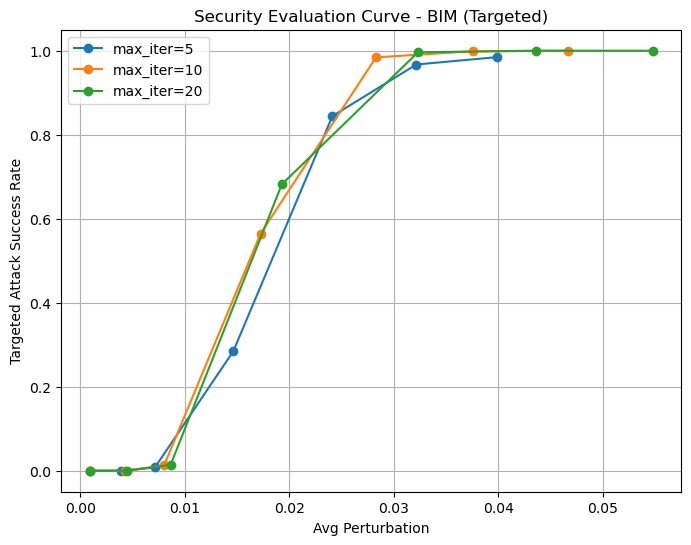
\includegraphics[width=0.75\textwidth]{images/evaluation_curve_bim_targeted.png}
                \caption{Security Evaluation Curve per l’attacco BIM in modalità targeted.}
                \label{fig:bim_targeted_curve}
            \end{figure}
            
            \noindent I risultati riportati in Figura~\ref{fig:bim_targeted_curve} mostrano un comportamento estremamente interessante: per valori bassi di \(\epsilon\) (\(\leq 0.005\)), l’attacco è inefficace indipendentemente dal numero di iterazioni, con un tasso di successo nullo. Ciò è dovuto al fatto che la distanza da percorrere per raggiungere una specifica classe bersaglio può richiedere modifiche più marcate rispetto al semplice inganno generico del classificatore. In questi casi, la rete neurale resiste bene a perturbazioni minime mirate.
            A partire da \(\epsilon = 0.01\), si inizia a osservare un lieve miglioramento, ma è solo con \(\epsilon \geq 0.025\) che l’attacco diventa significativamente efficace. In particolare, per \(\epsilon = 0.025\) e \texttt{max\_iter = 20}, il tasso di successo raggiunge il 68\%, crescendo poi rapidamente verso il 100\% con \(\epsilon = 0.075\) o superiore.
            Si nota inoltre come il numero di iterazioni gioca un ruolo cruciale: a parità di \(\epsilon\), passare da 5 a 20 iterazioni porta miglioramenti tangibili. Questo è coerente con la natura iterativa del BIM, che riesce a modellare gradualmente la perturbazione per renderla più efficace nel colpire la classe obiettivo.
            Infine, è importante osservare che l’alta efficacia dell’attacco non comporta necessariamente perturbazioni visivamente percepibili. Anche per \(\epsilon = 0.075\), la perturbazione media si aggira attorno a 0.04 (in scala normalizzata), dimostrando che l’avversario può ottenere una manipolazione mirata con alterazioni minime ma strategicamente dirette.

        \subsection{Projected Gradient Descent (Targeted)}
            Il \textit{Projected Gradient Descent} (PGD), nella modalità targeted, estende l’attacco BIM iterando piccoli passi verso la classe target e proiettando ad ogni passo l’immagine avversaria all’interno di una sfera $L\infty$ di raggio $\epsilon$ centrata sull’immagine originale:
            \[
            x_t = \Pi_\epsilon \left( x_{t-1} - \alpha \cdot \text{sign}( \nabla_x \mathcal{L}(h(x{t-1}, w), y_{\text{target}}) \right)
            \]
            
            \noindent dove $\Pi_\epsilon$ rappresenta la proiezione, $\alpha$ è lo step size definito come $\epsilon/5$ e $y_{\text{target}}$ è la classe desiderata.
            
            \begin{figure}[H]
                \centering
                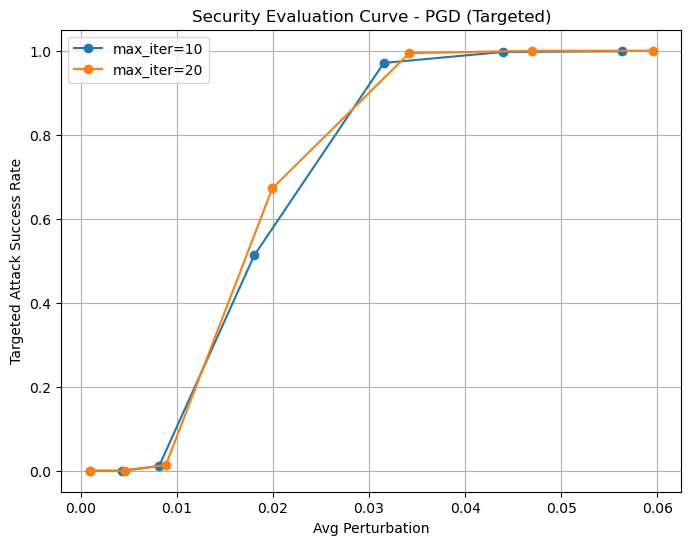
\includegraphics[width=0.75\textwidth]{images/evaluation_curve_pgd_targeted.png}
                \caption{Security Evaluation Curve per l’attacco PGD targeted, variando \texttt{max\_iter}.}
                \label{fig:pgd_targeted_curve}
            \end{figure}
            
            \noindent Come mostrato nella Figura~\ref{fig:pgd_targeted_curve}, PGD targeted è in grado di raggiungere un’elevata efficacia al crescere di \(\epsilon\), confermando la sua natura di attacco potente e controllabile. Per valori molto piccoli (\(\epsilon \leq 0.005\)), l'attacco fallisce nel condurre il classificatore verso la classe obiettivo, indipendentemente dal numero di iterazioni. Questo è un comportamento prevedibile, in quanto la distanza decisionale da colmare per passare a una classe specifica richiede modifiche più ampie rispetto al semplice errore di classificazione.
            Al crescere di \(\epsilon\), il successo aumenta in modo non lineare, si osserva infatti un punto di svolta attorno a \(\epsilon = 0.025\), dove il tasso di successo raggiunge il 50–67\%, e poi una rapida convergenza verso il 100\% già a \(\epsilon = 0.050\). L’impatto del numero di iterazioni è visibile ma limitato: 20 iterazioni permettono un attacco più efficace rispetto a 10 iterazioni, soprattutto nelle fasce intermedie di perturbazione.
            È interessante notare che l’attacco riesce a raggiungere un tasso di successo pressoché completo mantenendo una media di perturbazione ancora accettabile (\textasciitilde{}0.05), suggerendo che PGD sia in grado di costruire perturbazioni mirate ed efficaci, pur restando all’interno di soglie realistiche di impercettibilità visiva.
            Questa capacità di bilanciare efficacia e controllo fine del rumore rende PGD uno degli attacchi targeted più pericolosi tra quelli testati.

    \section{Carlini-Wagner L2 (Targeted)}
        L’attacco Carlini \& Wagner (CW) è noto per essere uno dei più efficaci nel contesto degli attacchi avversari, soprattutto nella modalità \textit{targeted}, dove l’obiettivo è forzare il modello a classificare un input come una specifica classe scelta. In questa sezione è stato implementato l’attacco CW-L2 in modalità targeted contro il modello NN1, variando i principali iperparametri di attacco per studiarne l’influenza sulla percentuale di successo e sull’entità della perturbazione.

        \subsection{Setup}
            Sono stati selezionati casualmente 20 campioni dal test set. Per ciascuno di essi è stata definita una classe target ciclica (\texttt{target = (label + 1) \% num\_classes}). Gli attacchi sono stati condotti variando:
            
            \begin{itemize}
              \item il \textbf{learning rate} ($lr \in \{0.01, 0.1\}$),
              \item il numero massimo di iterazioni ($max\_iter \in \{1, 10, 20\}$),
              \item la costante iniziale di bilanciamento tra obiettivo e perturbazione ($init\_const \in \{0.01, 0.1\}$).
            \end{itemize}

        \subsection{Risultati e Analisi}
            Il primo grafico (\autoref{fig:cw_l2_acc}) mostra l'\textbf{accuratezza targeted} in funzione del numero di iterazioni per diverse combinazioni di iperparametri. Si osserva chiaramente che:
                \begin{itemize}
                  \item L’aumento di \texttt{max\_iter} migliora significativamente il successo dell’attacco, a condizione che la costante iniziale non sia troppo bassa.
                  
                  \item La combinazione \texttt{lr=0.1} e \texttt{init\_const=0.1} consente di raggiungere il 100\% di successo già con sole 10 iterazioni, segno di una forte efficacia, ma anche di un possibile overfitting sulle immagini specifiche.
                \end{itemize}
            
            \begin{figure}[H]
                \centering
                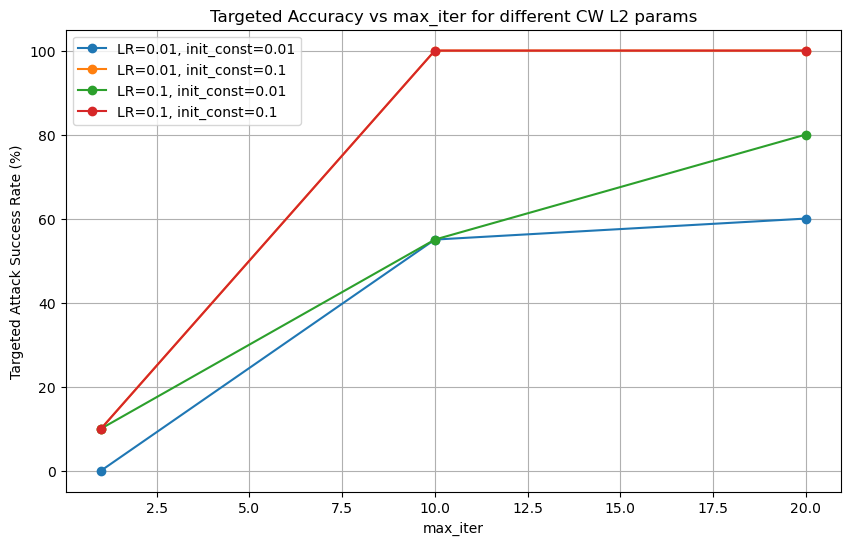
\includegraphics[width=0.75\textwidth]{images/cw_L2_accuracy_vs_maxiter.png}
                \caption{Targeted Attack Success Rate vs max\_iter per diverse combinazioni di parametri CW-L2}
                \label{fig:cw_l2_acc}
            \end{figure}
            
            \noindent Il secondo grafico (\autoref{fig:cw_l2_pert}) mostra l'\textbf{entità media della perturbazione} in norma $L_2$.
            In generale:
                \begin{itemize}
                  \item Le combinazioni con $init\_const=0.1$ inducono perturbazioni sensibilmente più alte, a discapito della stealthiness, ma a vantaggio della precisione.
                  
                  \item Le configurazioni con $lr=0.01$ mantengono perturbazioni più contenute, ma spesso richiedono più iterazioni per ottenere alti tassi di successo.
                \end{itemize}
            
            \begin{figure}[H]
                \centering
                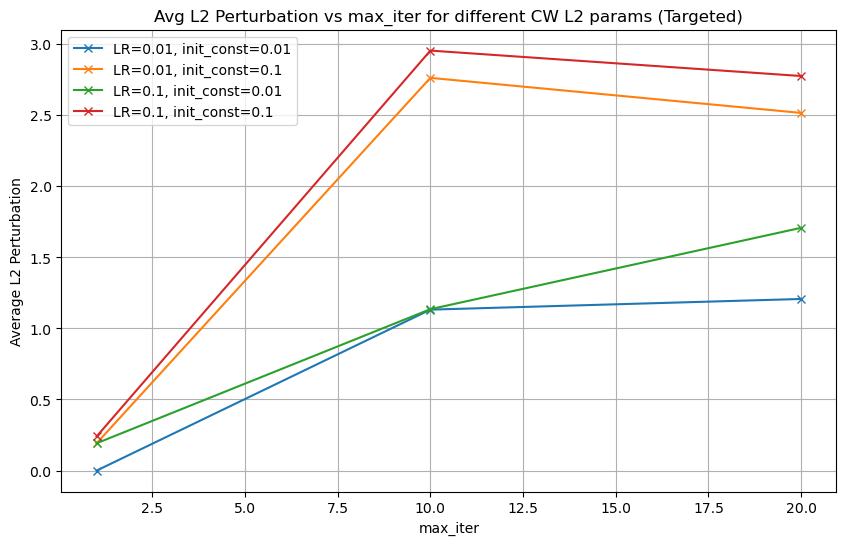
\includegraphics[width=0.75\textwidth]{images/cw_L2_perturbation_vs_maxiter.png}
                \caption{Average L2 Perturbation vs max\_iter per diverse combinazioni di parametri CW-L2}
                \label{fig:cw_l2_pert}
            \end{figure}
            
            \noindent Infine, la \textbf{Security Evaluation Curve} (\autoref{fig:cw_l2_sec}) mostra il trade-off tra efficacia e visibilità dell’attacco: all’aumentare della norma $L_2$, la percentuale di successo cresce in modo monotono, indicando una correlazione positiva tra aggressività e capacità di forzare la classificazione.
            
            \begin{figure}[H]
                \centering
                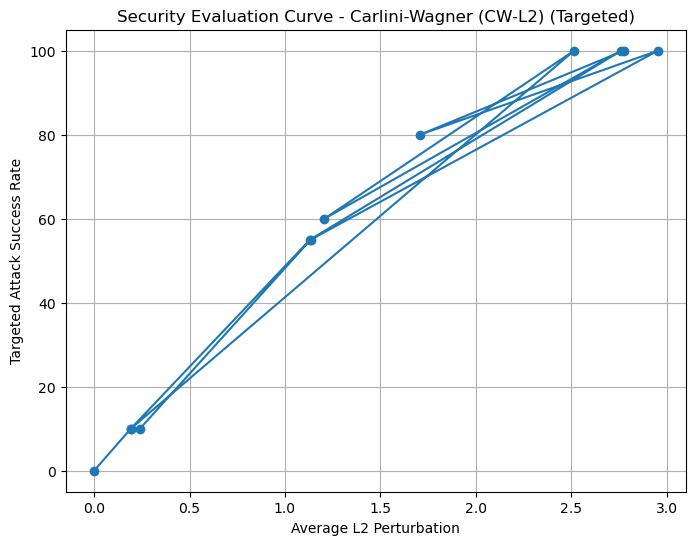
\includegraphics[width=0.65\textwidth]{images/cw_L2_security_curve.png}
                \caption{Security Evaluation Curve - Carlini \& Wagner (CW-L2) in modalità targeted}
                \label{fig:cw_l2_sec}
            \end{figure}

        \subsection{Osservazioni}
            Il raggiungimento del 100\% di successo in molte configurazioni non è anomalo per questo tipo di attacco, ma va interpretato con cautela: il CW-L2 è un attacco ottimizzativo potente, ma lavora su un piccolo subset di dati (20 immagini) e sfrutta conoscenza completa del modello. Di conseguenza, i risultati riflettono un'efficacia teorica elevata, che potrebbe ridursi in scenari reali o su modelli differenti.

    \section{Carlini-Wagner $L\infty$ (Targeted)}
        In questo esperimento abbiamo valutato l’efficacia dell’attacco \textit{Carlini-Wagner $L\infty$} in modalità \textit{targeted}, utilizzando il modello NN1 come rete bersaglio. Sono stati testati diversi valori per i principali iperparametri dell’attacco: \texttt{learning\_rate} $\in \{0.01, 0.1\}$, \texttt{initial\_const} $\in \{0.01, 0.1\}$, e \texttt{max\_iter} $\in \{1, 10, 20\}$. L’obiettivo era osservare come la variazione di tali parametri influenzasse la \textit{Targeted Attack Success Rate} e la dimensione della perturbazione media generata.
        
        \subsection{Risultati sperimentali}
            I risultati sperimentali mostrano che l’attacco Carlini-Wagner in modalità \textit{targeted} con norma $L\infty$ non ha prodotto alcun successo nel forzare la rete NN1 a classificare gli esempi avversari nella classe obiettivo, difatti in tutte le configurazioni testate, il tasso di successo è rimasto pari a $0\%$. Sebbene in alcune impostazioni siano state riscontrate perturbazioni visibili (con norma $L\infty$ fino a 0.0999), queste non si sono rivelate sufficienti a influenzare le decisioni del classificatore nella direzione desiderata.
            Tale risultato non implica necessariamente che l’attacco CW-$L\infty$ sia inefficace in senso assoluto. Al contrario, come evidenziato nel lavoro originale di Carlini e Wagner, l’attacco richiede in genere un numero molto elevato di iterazioni (spesso tra le 100 e le 1000) per ottimizzare efficacemente la perturbazione nella metrica $L\infty$ in contesto \textit{targeted}. Nel nostro caso, per motivi legati ai vincoli computazionali e alla disponibilità di tempo, abbiamo limitato il numero di iterazioni a $\{1, 10, 20\}$, valore che si è rivelato insufficiente per ottenere risultati significativi.
            È importante sottolineare che l’attacco CW-$L\infty$ è strutturato e potenzialmente molto potente, ma la sua efficacia dipende fortemente da un tuning accurato dei parametri e da un budget computazionale elevato. In assenza di tali condizioni, l’ottimizzazione risulta incompleta e incapace di generare perturbazioni che raggiungano l’obiettivo di classificazione imposto. In questo contesto, l'apparente fallimento dell'attacco è da attribuirsi principalmente a una configurazione sperimentale conservativa e non a una limitazione teorica dell'approccio stesso.
            
    \section{Confronto tra gli Attacchi Targeted}
        I risultati ottenuti mostrano una marcata differenza in termini di efficacia tra gli attacchi targeted analizzati. Gli attacchi iterativi come BIM e PGD si sono dimostrati estremamente efficaci nel forzare la rete a classificare le immagini secondo le etichette obiettivo, raggiungendo tassi di successo superiori al 99\% con valori di $\epsilon$ moderati e un numero di iterazioni sufficientemente alto.
        Al contrario, FGSM targeted ha mostrato un'efficacia molto limitata: essendo un attacco single-step, le perturbazioni risultano troppo deboli per influenzare il comportamento del classificatore verso una classe specifica.
        Il metodo Carlini-Wagner, pur essendo noto per la sua efficacia in modalità non-targeted, non ha prodotto risultati utili nella configurazione targeted sul nostro campione. Questo è probabilmente dovuto alla complessità del loss utilizzato, alla difficoltà di ottimizzazione in spazi ad alta dimensione e alla dimensione ridotta del test set.